\chapter{Application à l'analyse descriptive d'un grand corpus}
\label{chap:demo}
Ce chapitre décrit des résultats d'analyses statistiques observés lors de l'application de la chaîne proposée (Figure \ref{fig:intro:pipeline-globale}) sur un corpus formé de la base CAPP de la \citet{dila2019capp} (+65k XML sur 1997-2019), et plus de 10k autres documents de cours d'appels. Le module d'extraction d'information (Figure \ref{fig:demo:module-extraction}) est un système qui comprend les modèles développés durant les expérimentations de cette thèse. 

%  une base du tribunal de commerce de Paris (300k MS DOC sur ?-?), 500k décisions collectées de Legifrance
%à CAPP\_20190805-214041.tar.gz et Freemium_capp\_global\_20180315-170000.tar.gz 

%\verb|wget -c --accept='*.tar.gz' -r  ftp://echanges.dila.gouv.fr/CAPP/|

\begin{figure}[!htb]
	\centering 
	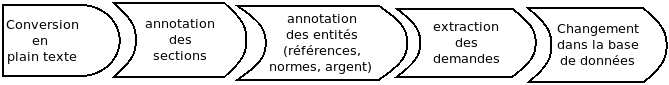
\includegraphics[width=0.8\textwidth]{pipeline-demo.png}
	\caption{Détails du module d'extraction d'information}\label{fig:demo:module-extraction}
\end{figure}

Après extraction, les décisions de la base de données sont réparties dans l'espace (ville) comme sur la figure \ref{fig:demo:doc-per-city} et dans le temps comme sur la figure \ref{fig:demo:doc-per-year}. Les demandes extraites se répartissent comme suit: 476 ACPA, 409 CONCDEL, 160 DANAIS, 0 DCPPC, 34 DORIS, et 45928 STYX.  

\begin{figure}[ht]
	\centering
	\begin{subfigure}[ht]{0.55\textwidth}
		\centering
		\centering
		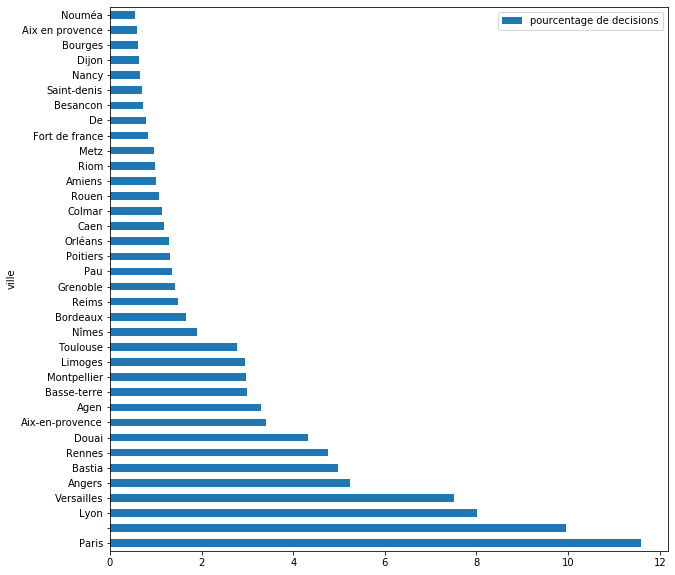
\includegraphics[width=\textwidth]{demo-pourcentage-decision-par-ville.png}
		\caption{Par ville (pourcentage>0)} \label{fig:demo:doc-per-city}
	\end{subfigure} 
	\begin{subfigure}[ht]{0.43\textwidth}
		\centering
		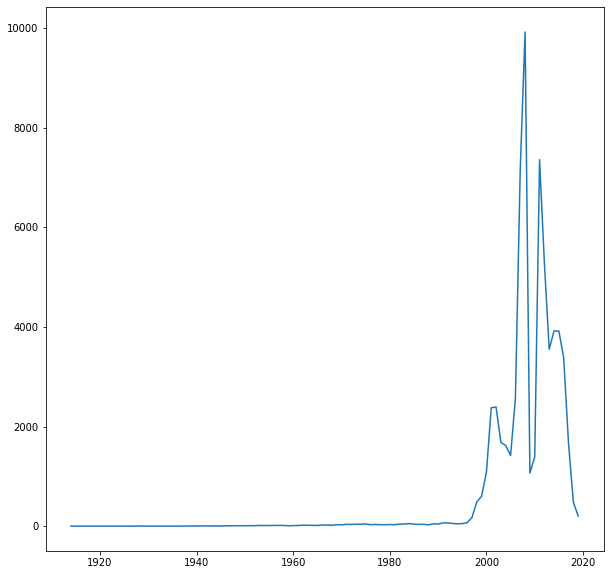
\includegraphics[width=\textwidth]{demo-repartition-decision-par-annee-1900_2019.png}
		\caption{Par an (entre 1900 et 2019)} \label{fig:demo:doc-per-year}
	\end{subfigure}
	\caption{Répartition des décisions} \label{fig:structuration:learning-curves}
\end{figure}


La structuration des données dans la base de données permet de mieux comprendre la jurisprudence à l'aide de graphiques appropriés. Une application de visualisation dédiée a notamment été développée  par \citet{PRYSIAZHNIUK2017jurisprudence-demo-web}.
Les analyses des sections suivantes sont restreintes aux 5 villes ayant les plus grands nombres de décision: Paris, Lyon, Versailles, Angers, Bastia; sur la période 2000-2019

\section{Analyse du sens du résultat}
A partir de la base des données extraites, l'évolution du pourcentage de demandes acceptées  peut être observée sur une courbe. En traçant une telle courbe pour chaque ville il est possible de comparer les villes.
Par exemple, pour les dommages intérêts sur l'article 700 du Code de Procédure Civile (STYX), la Figure \ref{fig:demo:analyse-sens-resultat-styx} compare l'évolution du sens du résultat entre les villes citées précédemment. On remarque que les demandes sont beaucoup plus rejetées qu'acceptées. La courbe du nombre total de demandes doit y être associée pour savoir si le pourcentage de succès est considérable\footnote{Pour une année où une seule demande est extraite et acceptée, le pourcentage est à 100\%, mais ce n'est pas considérable.}.

\begin{figure}[!htb]
	\centering 
	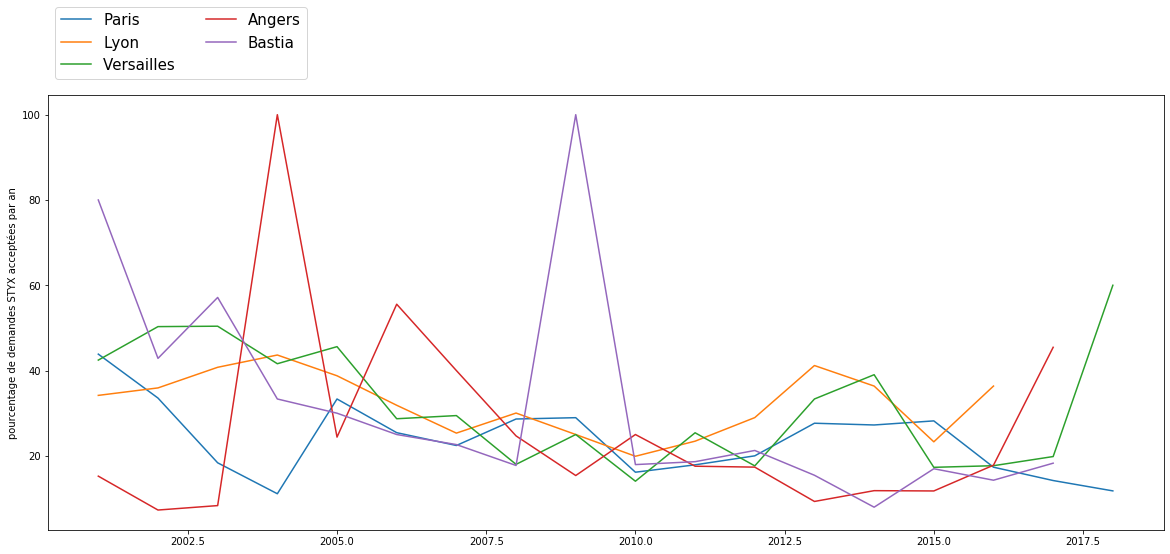
\includegraphics[width=0.9\textwidth]{evolution_sens_resultat_styx.png}
	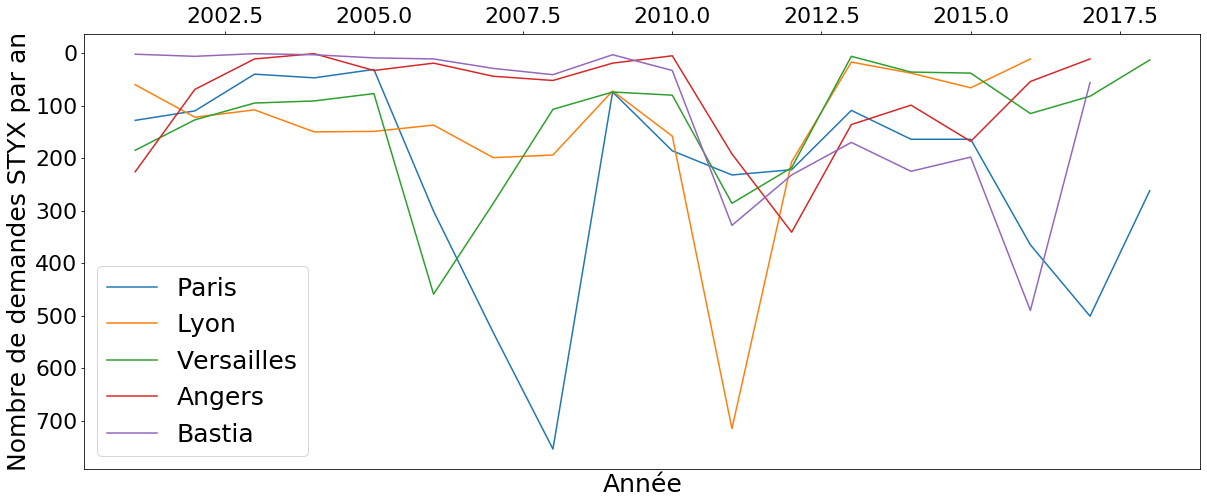
\includegraphics[width=0.9\textwidth]{evolution_nbdmd_styx.png}
	\caption{Evolution du sens du résultat des demandes STYX dans le temps à Paris, Lyon, Versailles, Angers, Bastia.}\label{fig:demo:analyse-sens-resultat-styx}
\end{figure}

La visualisation par l'application de \citet{PRYSIAZHNIUK2017jurisprudence-demo-web} permet de comparer les villes en observant sur un arbre l'épaisseur des branches associées aux catégories de demande (Figure \ref{fig:demo:web-styx}). On peut ainsi facilement observer quelles villes acceptent les demandes d'une certaine catégorie plus que d'autres par exemple.

% webdemo-sensresultat-5villes.png

\begin{figure}[!htb]
	\centering 
	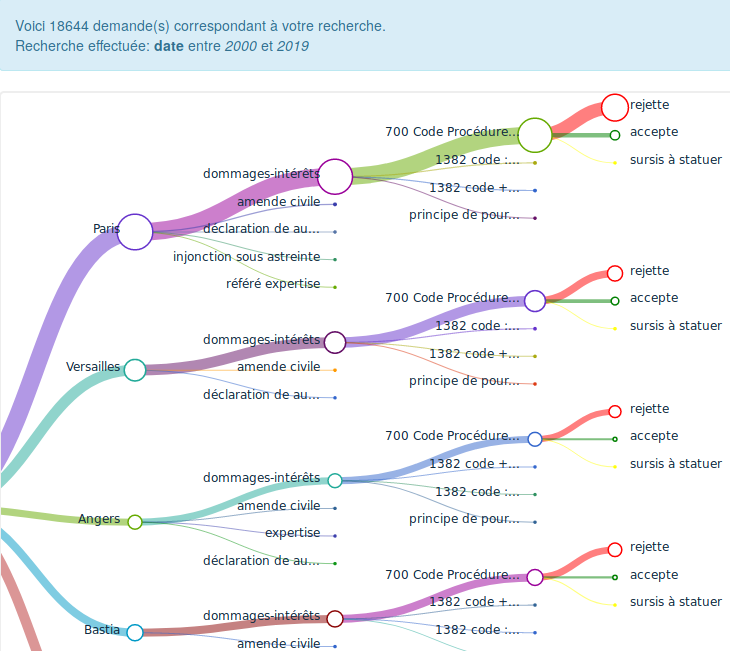
\includegraphics[width=0.6\textwidth]{webdemo-sensresultat-5villes.png}
	\caption{Comparaison des Paris, Lyon, Versailles, Angers, Bastia sur l'acceptation des demandes STYX à partir d'une visualisation arborée.}\label{fig:demo:web-styx}
\end{figure}

\section{Analyse des quanta}
\subsection{Evolution dans le temps}
De même l'évolution des quanta demandés et accordés peut être facilement visualisée par un diagramme en barre comme celui de la Figure \ref{fig:demo:evolution-quanta-styx} qui correspond aux demandes STYX entre 2000  et 2019. Même si le nombre total de demandes est à prendre en compte, un tel diagramme donne un aperçu des sommes d'argent demandés et accordés chaque année. 

\begin{figure}[!htb]
	\centering 
	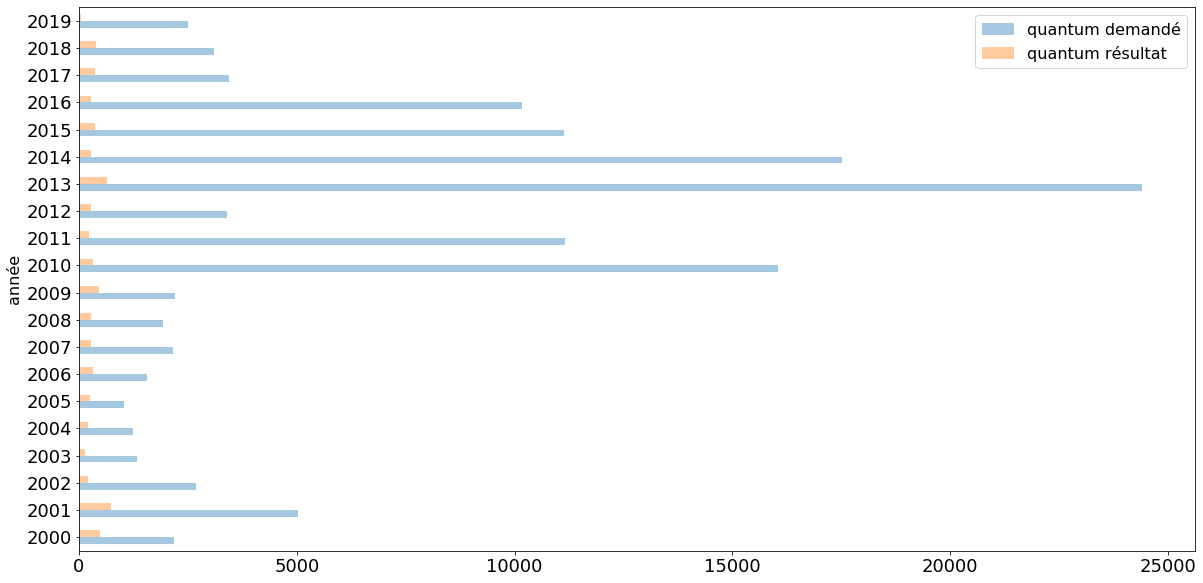
\includegraphics[width=0.8\textwidth]{evolution_quanta_styx.png}
	\caption{Evolution des quanta moyens par année des demandes STYX entre  2000  et 2019.}\label{fig:demo:evolution-quanta-styx}
\end{figure}


\subsection{Différence dans l'espace}

Pour avoir une idée du montant qu'on peut recevoir pour une catégorie de demande, l'évolution des valeurs généralement accordés peut être comparée entre deux villes en visualisant les diagrammes boîtes (\textit{boxplot}) 
des quanta accordés dans ces villes. La Figure \ref{fig:demo:evolution-qr-styx-compare-ville} permet d'effectuer une comparaison entre Bastia et Lyon. On remarque, par exemple, qu'en cas d'acceptation de la demande, il faut s'attendre à recevoir au maximum une somme autour de 5k euros à Bastia contre 10k euros à Lyon.

\begin{figure}[!htb]
	\centering 
	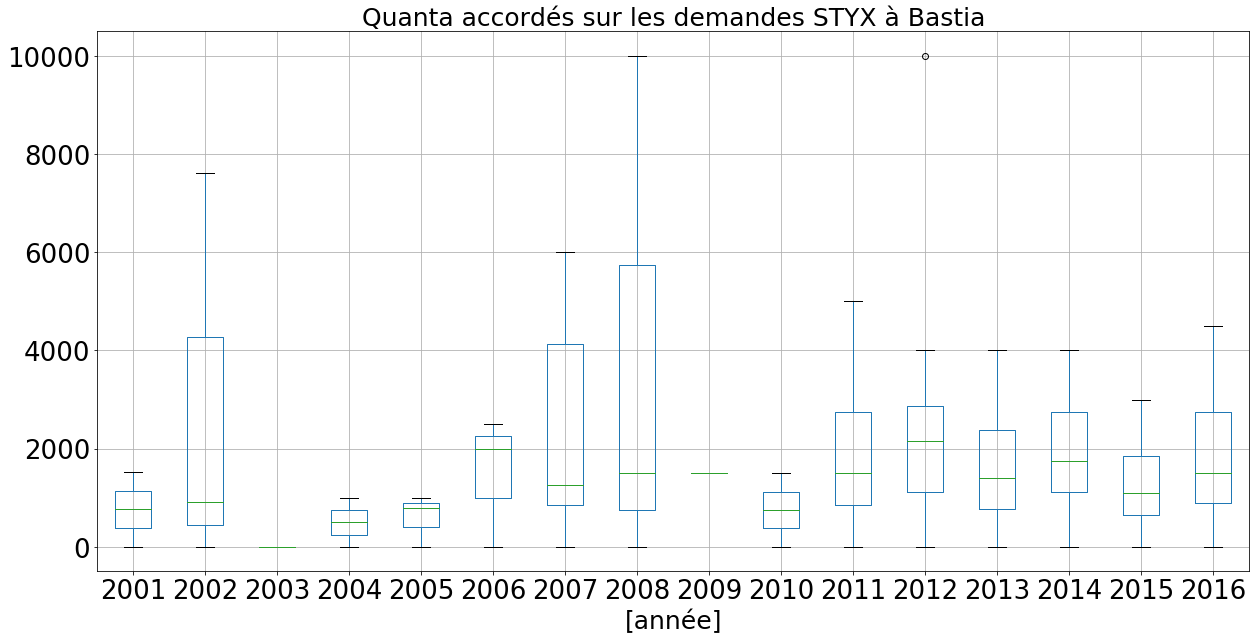
\includegraphics[width=0.6\textwidth]{qr_STYX_Bastia.png}
	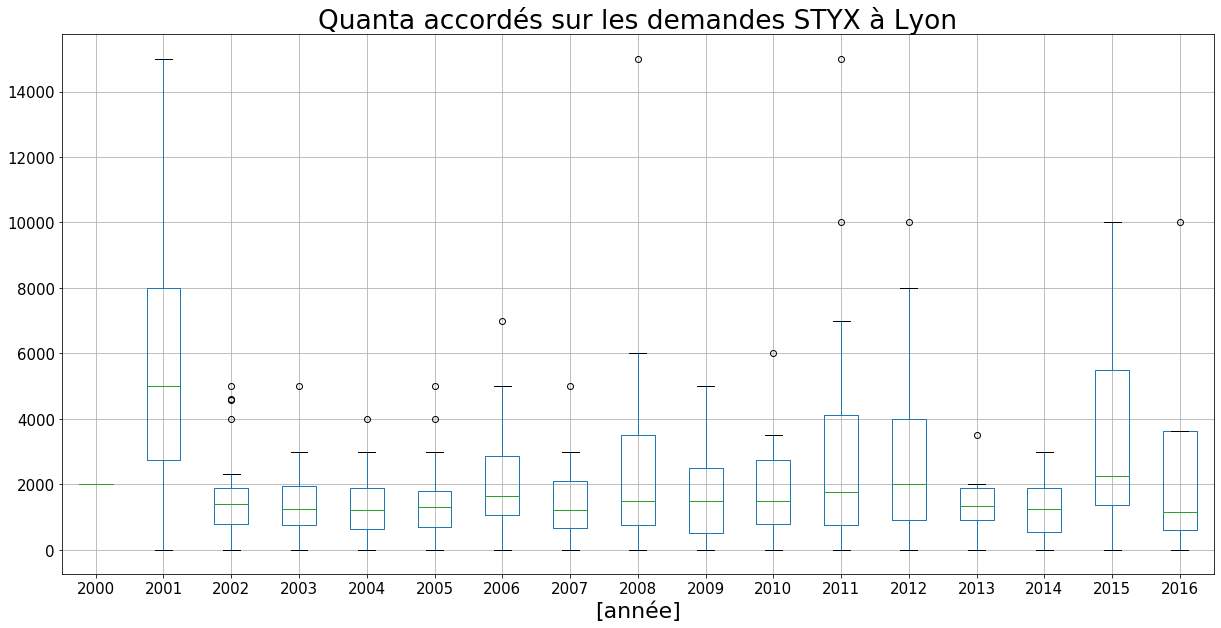
\includegraphics[width=0.6\textwidth]{qr_STYX_Lyon.png}
	\caption{Evolution des quanta accordés par année sur les demandes STYX entre 2000 et 2016 à Bastia et à Lyon.}\label{fig:demo:evolution-qr-styx-compare-ville}
\end{figure}


\subsection{Quantum demandé vs. quantum accordé}
La prédiction du quantum résultat doit définir un modèle dont la forme s'accorde avec celle du nuage de points ($x=$ quantum demandé, $y=$ quantum accordé) correspondant. D'après les nuages de points observés pour Paris, Bastia, Angers et Lyon (Figure \ref{fig:demo:qr-vs-qd-styx-compare-ville}), le quantum demandé ne semble pas suffisant seul pour déterminer le quantum accordé\footnote{Différentes valeurs de quantum résultat sont observées pour la même valeur de quantum demandé.}. Il sera ainsi nécessaire de tenir compte des circonstances factuelles et autres spécificités du cas traité qui permettront de filtrer les décisions sur lesquelles se basera l'apprentissage. On remarque néanmoins une ressemblance de forme entre les nuages de points des différentes villes. 

\begin{figure}[!htb]
	\centering 
	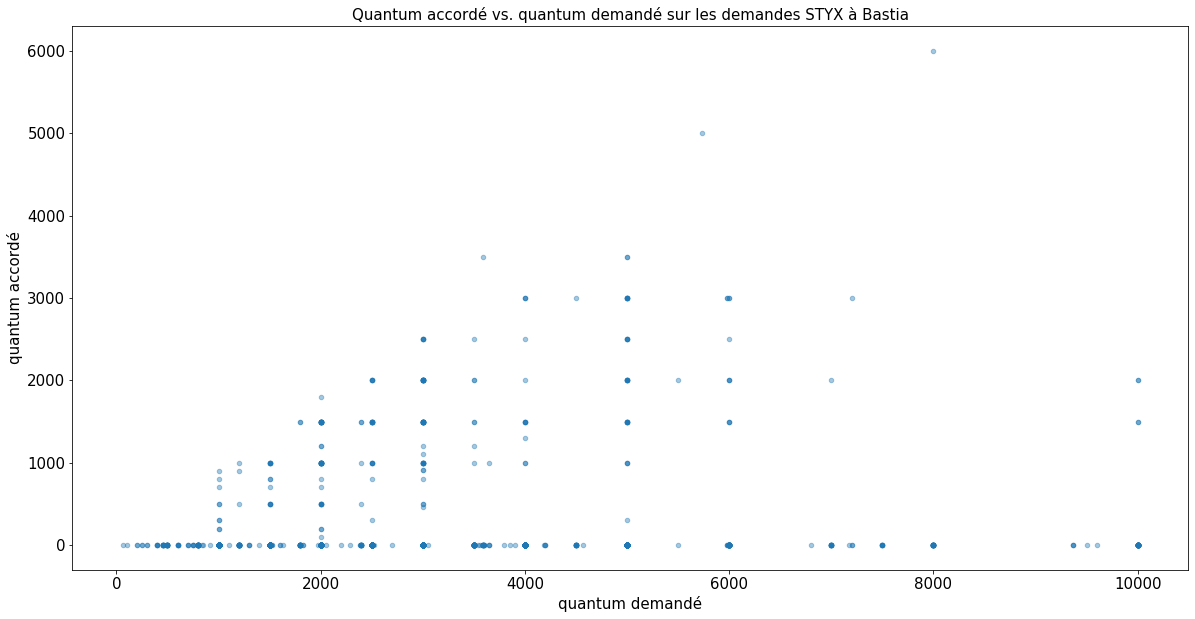
\includegraphics[width=0.47\textwidth]{qr-vs-qd_STYX_Bastia.png}
	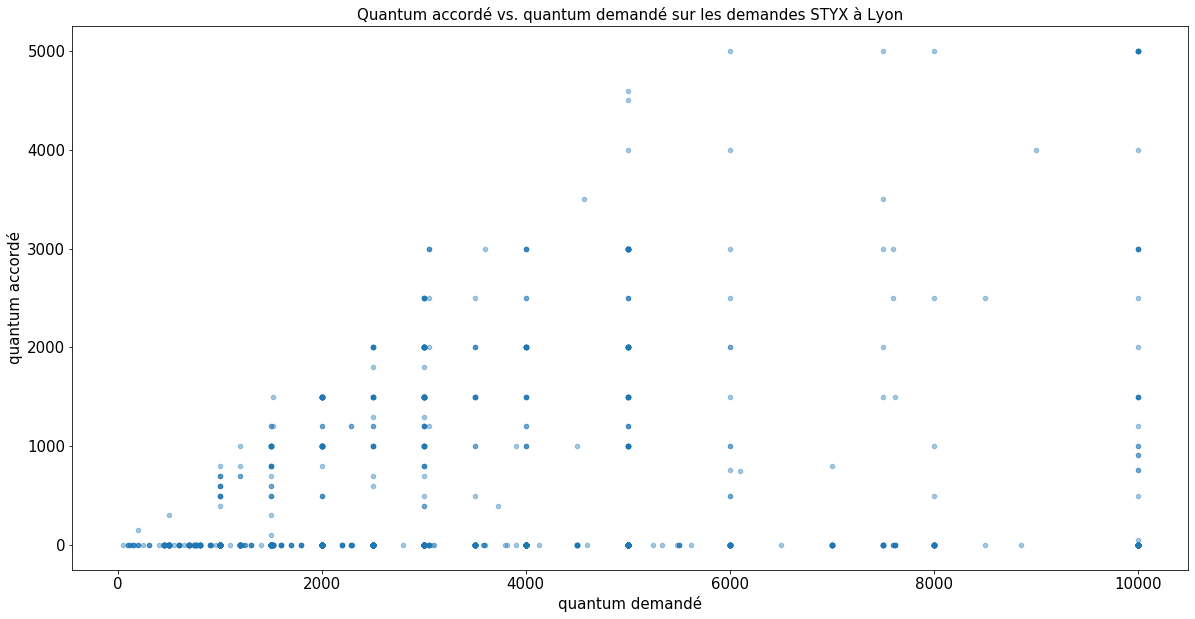
\includegraphics[width=0.47\textwidth]{qr-vs-qd_STYX_Lyon.png}
	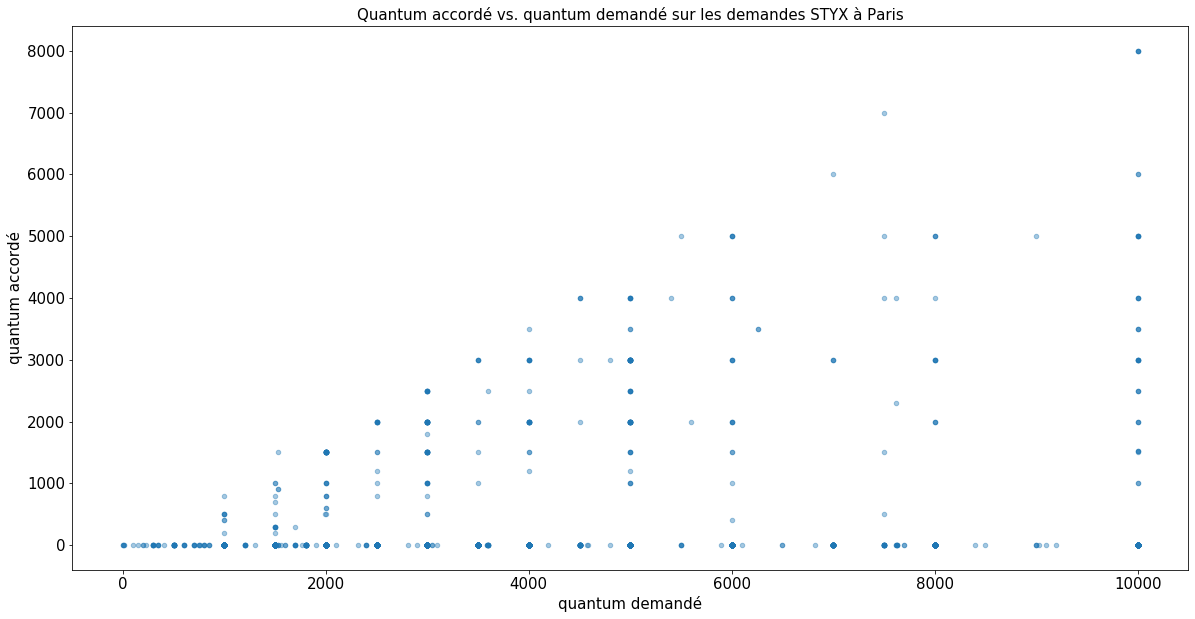
\includegraphics[width=0.47\textwidth]{qr-vs-qd_STYX_Paris.png}
	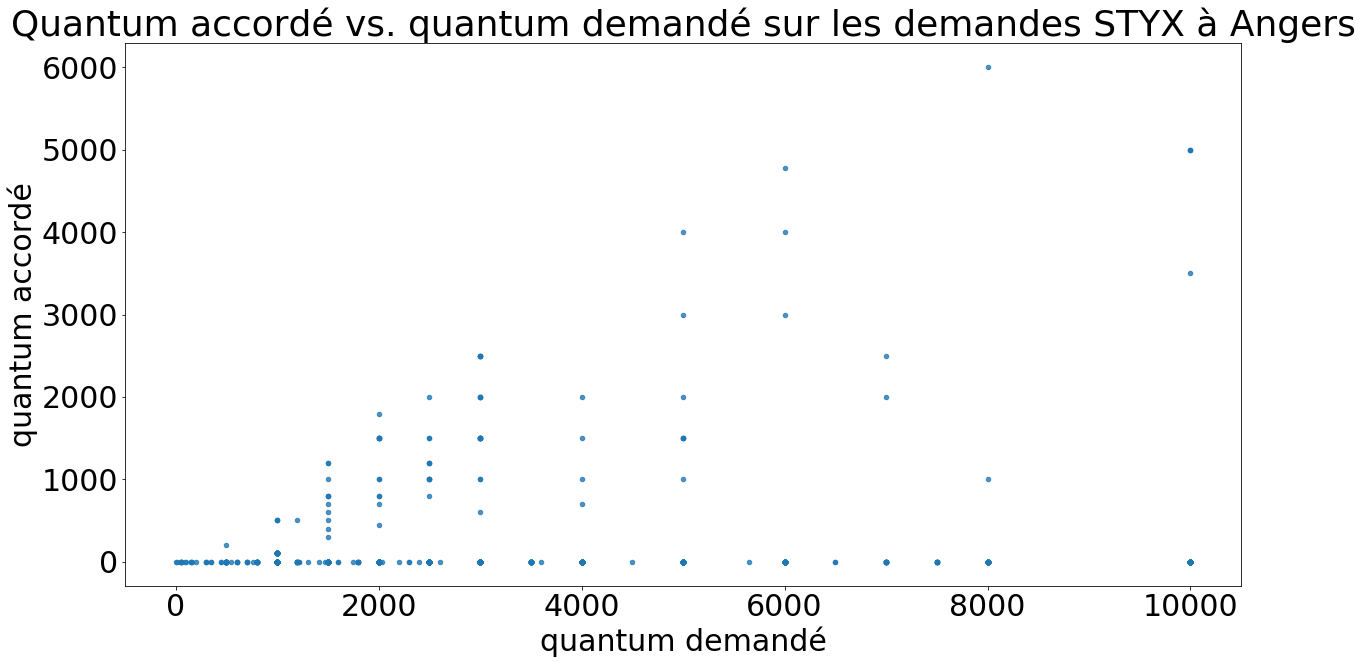
\includegraphics[width=0.47\textwidth]{qr-vs-qd_STYX_Angers.png}
	\caption{Nuages des points (quantum accordé, quantum demandé) pour les demandes STYX entre 2000 et 2019 à Paris, Bastia, Angers et Lyon (quantum demandé < 10000) .}\label{fig:demo:qr-vs-qd-styx-compare-ville}
\end{figure}

\section{Conclusion}
\label{sec:demo:conclusion}
Les démonstrations de ce chapitre donnent quelques exemples de statistiques qui informent de l'état de la jurisprudence à partir d'informations extraites à l'aide des approches proposées dans cette thèse. Les analyses du sens du résultat et des quanta sont les principales applications directes de la chaîne de traitement développée. Ce chapitre se limite aux filtres sur l'année, la ville, et la catégorie de demande, mais les analyses peuvent déjà être affinées en associant d'autres filtres comme  des mot-clés,  les normes appliqués, ou le type de juridiction. Les analyses pourront être plus riches grâce l'extraction future de nouvelles informations comme les motivations des juges et de meilleurs modèles de circonstances factuelles.